\section{Test Plan}
In order to test the effectiveness of the filter the mathematical limits given by the size of the input and on the coefficient values had to be tested.
To ease the testing of the filter with different inputs the test bench reads/writes data from/to file.
\subsection{Size limits}
To stress out the size limits computed in section \ref{sec:sizing} the filter has been feeded with maximum value in modulus i.e. ($-2^(b-1)= -32768 $) repeated continuosly and checked if the output corresponded to the value given by applying in Matlab expression \ref{eq:general}, the results can be seen in the following figure:
\begin{figure}[H]
  \centering
  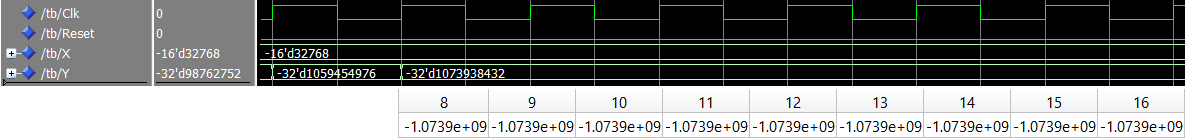
\includegraphics[width=0.9\linewidth]{./images/simul32768.PNG}
  \caption{Testbench of the filter with -32768 as costant input}
  \label{fig:32768}
\end{figure}
The network at regime settles to 1073938432 that corresponds to the value returned by Matlab.
\subsection{Cut-off frequency}